\documentclass[crop,tikz]{standalone}

\usepackage{verbatimbox}
\usepackage{listings}
\lstset{basicstyle = \small\ttfamily}
\usepackage{graphicx} % more modern
\usetikzlibrary{fit}
\usetikzlibrary{arrows.meta}
\usetikzlibrary{positioning}
\usetikzlibrary{decorations.text,decorations.pathreplacing}
\usetikzlibrary{decorations.pathmorphing}

\begin{document}









  \begin{tikzpicture}
  \node[ thick,anchor = west,inner sep=0pt,label={[yshift = 0.3cm]{\small \begin{tabular}{c}
          \textbf{Image}\\
          \textbf{(Observed)}
  \end{tabular}}}](observation) at (0,0) {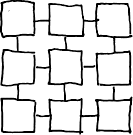
\includegraphics[width = 1.5cm]{figures/expert-39-trimmed.png}};
    \node[ultra thick,anchor = west,inner sep=0pt](traceSource) at (3.7,0.5){    \begin{lstlisting}[basicstyle = \scriptsize\ttfamily]
line, line,
rectangle,
line, ...
\end{lstlisting}};
    \node[ultra thick,anchor = west,inner sep=0pt](traceImage) at (4,-0.5) {
      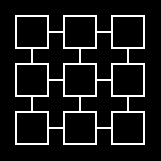
\includegraphics[width = 0.9cm]{figures/39-parse.png}}; 
    \node(trace)[draw,thin,fit = (traceImage) (traceSource), label = above:{{\small \begin{tabular}{c}
            \textbf{Spec/Drawing Commands}\\
            \textbf{(Latent)}
    \end{tabular}}}] {};
    
    \node[draw, thick,anchor = west,inner sep=2pt,label=above:{\small \begin{tabular}{c}
          \textbf{Program}\\
          \textbf{(Latent)}
    \end{tabular}}](program) at (7.7,0) {
      \begin{lstlisting}
for (j < 3)
for (i < 3)
if (...)
 line(...)
 line(...)
rectangle(...)
    \end{lstlisting}};
    \node[ultra thick,anchor = west,inner sep=0pt,label=below:{\small Extrapolation}](extrapolate) at (12,1) {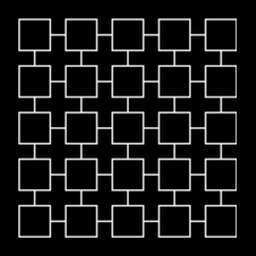
\includegraphics[width = 1.3cm]{figures/39-extrapolated.png}};
%    \node[ultra thick,anchor = west,inner sep=0pt,label=below:{\small Similarity}](similarity) at (11.3,0) {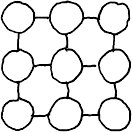
\includegraphics[width = 1cm]{figures/expert-38-trim.png}};
    \node[ultra thick,anchor = west,inner sep=0pt](errors) at (12.1,-1) {\begin{tabular}{l}
        \small Error \\\small correction
    \end{tabular}};

    \draw[->, ultra thick] ([yshift=10]trace.west) to[out = 150,in = 30] node[midway,yshift = 6]{{\small Rendering}} ([xshift=5,yshift=10]observation.east); % -- node[fill = white,rotate = -90] {{\small Rendering}}
    \draw[->, very thick, red] ([yshift = -15,xshift=3]observation.east) to[out = -30,in = -150] node[midway,yshift = -12,xshift=5]{{\small \begin{tabular}{l}
          Learning + \\Stochastic search
    \end{tabular}}} ([yshift = -15]trace.west);
    \draw[->, ultra thick] ([yshift=10]program.west) to[out = 150,in = 30] node[midway,yshift = 6] {{\small Execution}} ([yshift=10]trace.east);
    \draw[->, very thick, red] ([yshift = -15,xshift=0]trace.east) to[out = -30,in = -150] node[midway,yshift = -12,xshift=9]{{\small \begin{tabular}{l}
          Learning + \\Program synthesis
    \end{tabular}}} ([yshift = -15]program.west);

%    \draw[->, thick, red, very thick] ([xshift = 10]trace.south) to[out = -10,in = -170] node[midway,yshift = -6]{{\small Learning + Program synthesis}} ([xshift = 10]program.south);
    \draw[->, very thick, red] (program.east) to[out = -60,in = 180] (errors.west);
%    \draw[->, thick] (program.east) to[out = 40,in = -230] (similarity.west);
    \draw[->, thick, red, very thick] (program.east) to[out = 60,in = 180] (extrapolate.west);

    \draw[decoration = {brace,mirror,raise = 5pt},decorate,thick]
    ([yshift = -11,xshift = -130]trace.south) -- node[below = 6pt] {{\small  Image$\to$Spec}} ([yshift = -11,xshift = -5]trace.south);
    \draw[decoration = {brace,mirror,raise = 5pt},decorate,thick]
    ([xshift = 5,yshift = -11]trace.south) -- node[below = 6pt] {{\small  Spec$\to$Program}} ([xshift = 170,yshift = -11]trace.south);
    \draw[decoration = {brace,mirror,raise = 5pt},decorate,thick]
([xshift = 180,yshift = -11]trace.south) -- node[below = 6pt] {{\small  Applications}} ([xshift = 255,yshift = -11]trace.south);
  \end{tikzpicture}
\end{document}
